\documentclass{beamer}
\usetheme{metropolis}           % Use metropolis theme
\usepackage[utf8]{inputenc}
\usepackage[brazil]{babel}
\usepackage{soul}
\usepackage{float}
\usepackage{caption}
\usepackage{subcaption}
\usepackage[style = abnt, backend = biber]{biblatex}
\addbibresource{refs.bib}
\title{Emergência de Distribuições de Preferência no caso Unidimensional: uma
  abordagem computacional}
\date{}
\author{Marcelo Veloso Maciel}
\institute{}
\begin{document}
\maketitle



% ----------------- NOVO SLIDE --------------------------------
\begin{frame}{Sumário}
\tableofcontents
\end{frame}



\section{Introdução}
\begin{frame}{Objetivo}
  Propor e analisar um modelo generativo de Opinião Pública
\end{frame}


\begin{frame}{Justificativa}
  \begin{itemize}
  \item Normativa
  \item Positiva
  \end{itemize}
\end{frame}

\begin{frame}{Escopo}
  \begin{itemize}
  \item Sistema Alvo \(\rightarrow\) Opiniões Públicas Nacionais
  \item Microfundamentos da Opinião Pública = Opinião Idiossincrática +
    Influência Social (Pares e \st{Mídia} )
  \end{itemize}
  
\end{frame}

\section{Fundamentação Teórica}
\begin{frame}{Literaturas}

Critérios de Fidelidade \cite{weisberg2012simulation}:
\begin{itemize}
\item Estrutura;
\item \textit{Output}.
\end{itemize}
  
Base para a construção do modelo:

\begin{itemize}
\item Teoria Política Formal
\item Dinâmicas de Opinião
\item \textcolor{gray!70}{Opinião Pública}
\end{itemize}
\end{frame}

\begin{frame}{Teoria Política Formal}

  \begin{itemize}
  \item Definição: Modelagem Formal de Política;
  \item Principal subconjunto: Teoria da Escolha Racional;
  \item Modelo do ator racional: Preferências e Crenças Consistentes + Atualização
    Bayesiana.
  \end{itemize}

\end{frame}


\begin{frame}{Teoria Espacial e Eleições: Microfundamentos I}
  \begin{itemize}
  \item Teoria Política Espacial : analogia espacial;
  \item Comitês x Eleições de Larga Escala;
  \item Atitudes e  Ideologia.
  \end{itemize}
\end{frame}

\begin{frame}{Teoria Espacial e Eleições: Macrofundamentos I }
  \begin{itemize}
\item \textcite{druckman2012public} aponta dois achados canônicos da Opinião
  Pública:
  \begin{itemize}
  \item Instabilidade Micro;
  \item Estabilidade Macro.
  \end{itemize}
  \end{itemize}
  
\end{frame}


\begin{frame}{Teoria Espacial e Eleições: Macrofundamentos I }
  \begin{figure}[H]
    \centering
    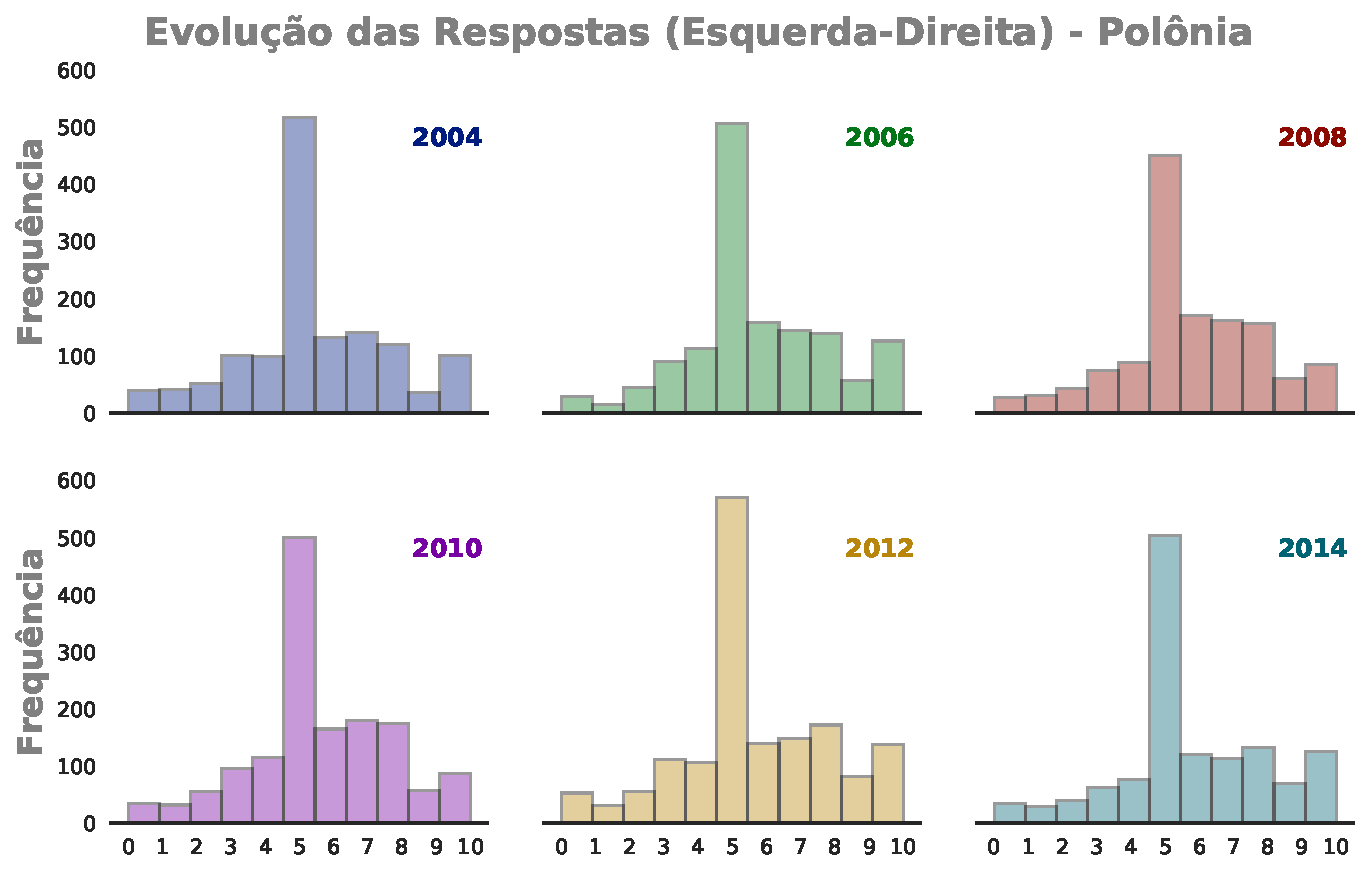
\includegraphics[scale = 0.4]{ims/ess_Pol_plots.pdf}
    \caption{Estabilidade Ideológica}
    \label{fig1}
  \end{figure}
\end{frame}


\begin{frame}{Teoria Espacial e Eleições: Macrofundamentos II}

  \begin{itemize}

  \item Partidos e Relevo Eleitoral
 \item \textcite{flache2017} aponta os seguintes fatos estilizados sobre
   distribuições de opinião pública no ESS:
   
    \begin{itemize}

    \item  há um pico central dominante;
    \item há uma tendência para a existência de \textit{clusters} não centrais;
    \item há uma tendência a picos nos extremos.
      
    \end{itemize}
    
  \end{itemize}
  
\end{frame}

\begin{frame}{Teoria Espacial e Eleições: Macrofundamentos II}  
  \begin{figure}[H]
      \centering 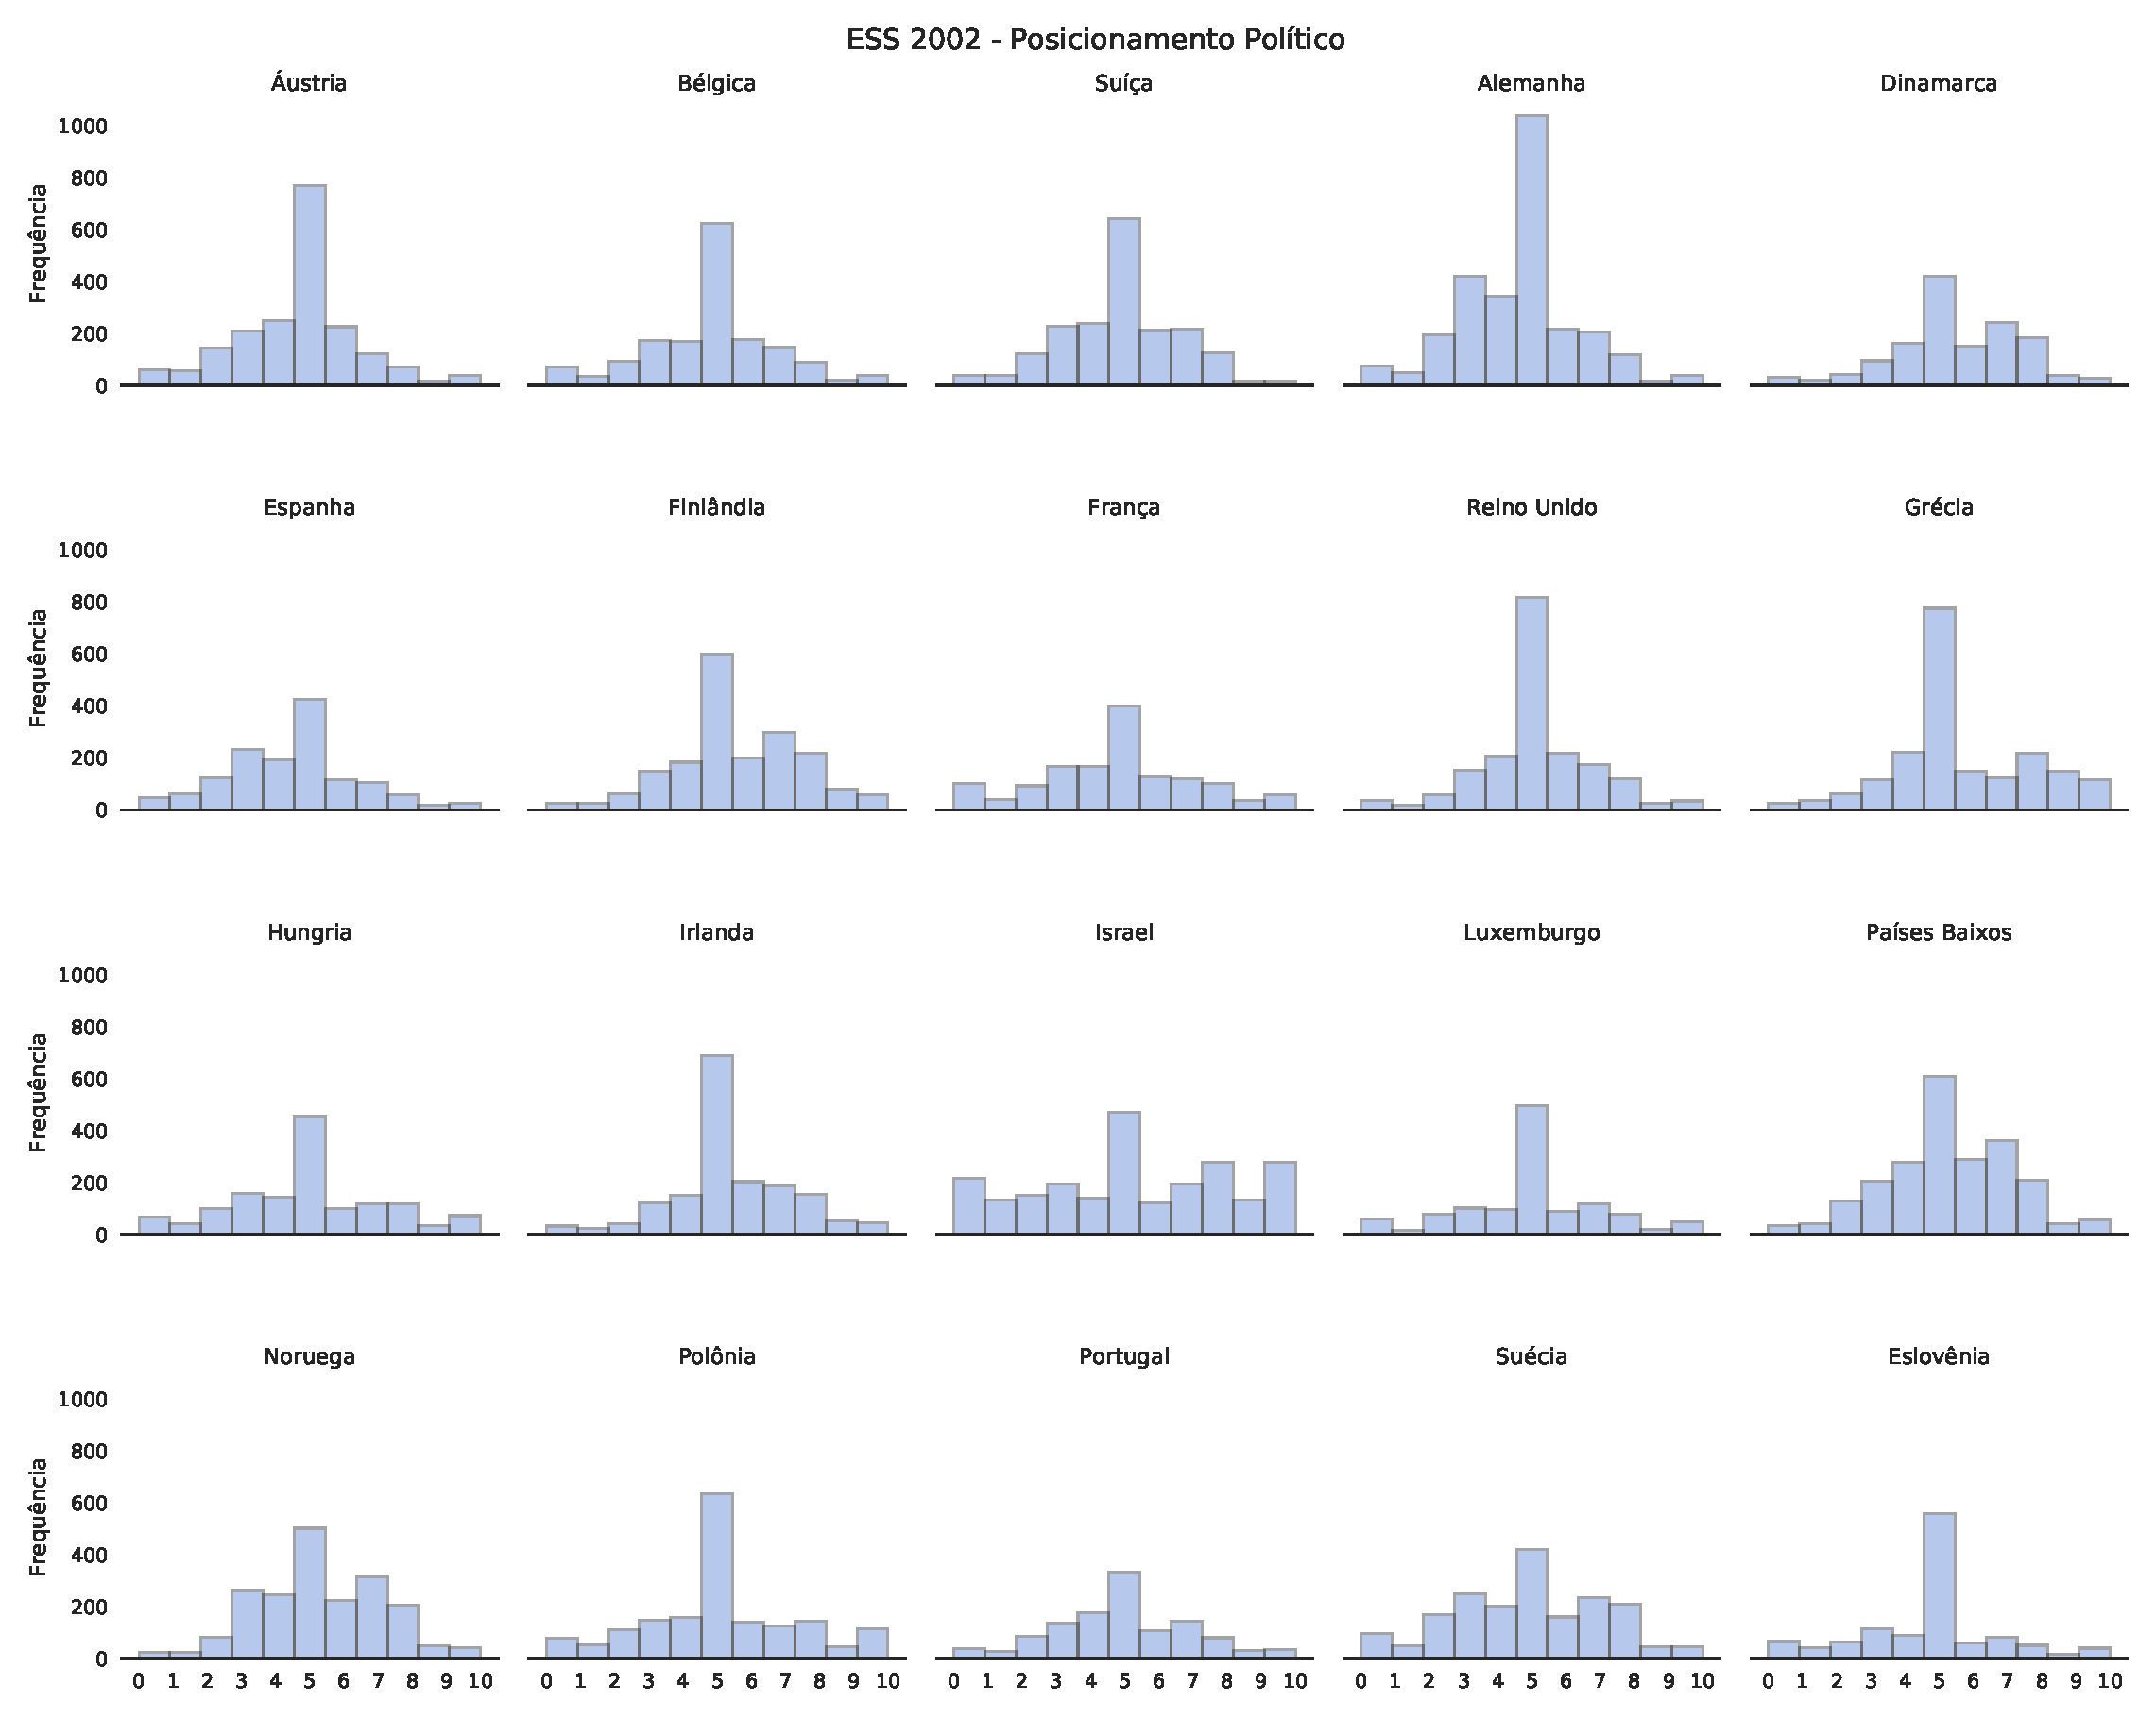
\includegraphics[scale = 0.2]{ims/ess_2002_plots.pdf}
    \caption{ Distribuição de Posicionamento Ideológico de respondentes em 20
      países}
    \label{fig2}
  \end{figure}
\end{frame}


\begin{frame}{Dinâmicas de Opinião}
  \begin{itemize}
  \item Definição de OD;
  \item Modelagem Baseada em Agentes;
  \item Estrutura de um modelo de OD:
    \begin{itemize}
    \item Os agentes têm as seguintes propriedades:

      \begin{itemize}
      \item Opinião;
      \item Estrutura de Interação (topologia + regra de interação);
      \item Regra de Atualização;
      \end{itemize}
    \item Três classes \cite{flache2017}:
      \begin{itemize}
      \item Modelos de Influência Social Assimilativa;
      \item Modelos com influência enviesada  \(\leftarrow\) viés partidário;
      \item Modelos de influência repulsiva.
      \end{itemize}
      
    \end{itemize}
  \end{itemize}
\end{frame}

\begin{frame}{Modelos Canônicos em OD}
  \begin{itemize}
  \item Inspirado em Ising;
  \item Voter;
  \item Regra da Maioria;
  \item Sznajd;
  \item Axelrod
  \item Deffuant-Weisbuch
  \end{itemize}
\end{frame}

\begin{frame}{OD e Espectro Cognitivo }
  \begin{itemize}
  \item Arquiteturas Cognitivas \(\longleftrightarrow\) Modelos Fisicalistas
  \item Arquiteturas Cognitivas \(\rightarrow\) ``Maldição da Dimensionalidade''
    \cite{de2005computational}
  \item Modelos Fisicalistas \(\rightarrow\) Modelagem ad-hoc
  \end{itemize}
\end{frame}

\begin{frame}{Espectro Cognitivo e Modelos Bayesianos}
  \begin{itemize}
  \item Agentes Imperfeitamente Bayesianos: ``meio termo virtuoso''
  \item Framework de \textcite{martins2012bayesian};
  \item \textcite{martins2009bayesian} aplicação para um espaço contínuo:
    \begin{itemize}
    \item    \( o_i(t+1)
    =
    p
    \frac{o_i(t) + o_j(t)}{2}
    +
    (1-p^*)o_i(t) \)
    \item \(    \sigma_i^2(t+1)
    =
    \sigma_i^2(t)
    (1 - \frac{p^*}{2})
    +
    p^*
    (1-p^*)
    (\frac{o_i(t)-o_j(t)}{2})^2\)
    \end{itemize}
  \end{itemize}
\end{frame}

\begin{frame}{OD : Microfundamentos II}
  \begin{itemize}
  \item Regra de Interação: \(ij\);
  \item Regra de Atualização : assimilação enviesada imperfeitamente bayesiana
    (viés partidário);
  \end{itemize}
\end{frame}

\section{Modelo e Resultados Parciais}
\begin{frame}{Proposta de Modelo}
  \begin{itemize}
  \item Agentes têm um \textit{perfil ideológico} que é o conjunto de crenças
    deles sobre questões;
  \item Cada crença deles sobre questões segue o framework de
    \textcite{martins2012bayesian};
  \item O posicionamento na dimensão, seu ponto ideal, é dado pela média das
    opiniões em cada questão;
  \item A regra de atualização é a mesma que \textcite{martins2009bayesian}: a
    cada interação os agentes atualizam a crença sobre \textit{uma} das
    questões;
  \item A regra de interação é entre pares;
    \item Topologia?
  \end{itemize}
\end{frame}

\begin{frame}{Implementação I}

Os parâmetros-chave para configuração do modelo são:
\begin{itemize}
\item A população de \(500 < N < 10000\) agentes;
\item O número de questões \(1 \leq n \leq 10\); 
\item As opiniões \(0.0< o_i< 1.0\) dos agentes
  \begin{itemize}
  \item A opinião dos agentes no tempo \(t = 0\) é retirada de uma distribuição
    uniforme;
  \end{itemize}
\item As incertezas \(0.01 \leq \sigma_i \leq 0.5\);
  \begin{itemize}
  \item A incerteza é, na condição inicial, a mesma para todos os agentes;
  \item Vamos considerar versões em que os agentes atualizam as incertezas e que
    não atualizam.
  \end{itemize}

\item O parâmetro de confiança \(0.1 \leq p \leq 0.99\);
  \begin{itemize}
  \item Vamos considerar variantes em que o \(p\) é global ou em que o \(p\) é
    calculado para cada interação;
  \end{itemize}
  
\item A probabilidade de reconsideração \(0.0 \leq \rho  \leq 0.1\);
  \begin{itemize}
  \item Vamos considerar casos com e sem ruído.
  \end{itemize}
\end{itemize}
\end{frame}


\begin{frame}{Implementação II - Resultados Parciais}

Implementei a simulação:
\begin{itemize}
  \item N = 500;
\item em um grafo completo;
\item  com 1,5 ou 10 questões;
\item com \textit{todos} os agentes atualizando suas opiniões (somente, não a incerteza);
\item com \(p\) global de 0.1, 0.3, 0.7 e 0.9 ; 
\item com \(\sigma\) de 0.02, 0.05, 0.1 e 0.3;
  \item com \(\rho\) de 0.0, 0.0001, 0.001, 0.01 e 0.1.
\end{itemize}
\end{frame}

\begin{frame}{Resultados Parciais - Sobre \(\rho\)}
   \(\rho = 0.01 \) e \(0.1 \) dominam o comportamento do modelo, em especial
   quando \(n = 1\).
   
\end{frame}




\begin{frame}{Resultados Parciais - Sobre \(\rho\)}
  
  \begin{figure}[H]
    \centering
    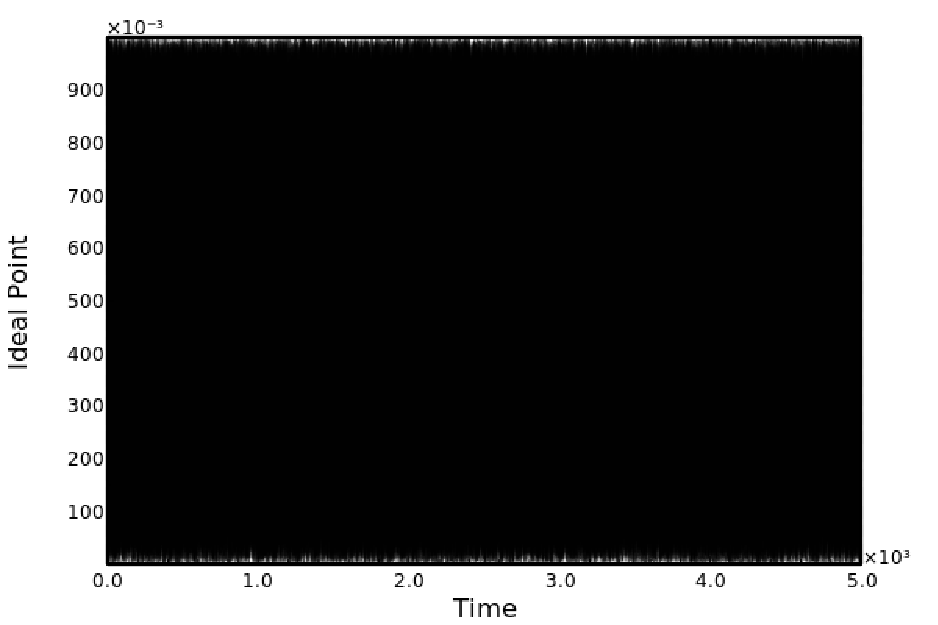
\includegraphics[scale = 0.5]{ims/rho01.pdf}
    \caption{\(\rho = 0.1\)}
  \end{figure}
\end{frame}


\begin{frame}{Resultados Parciais - Sobre \(\rho\)}
  
  \begin{figure}[H]
    \centering
    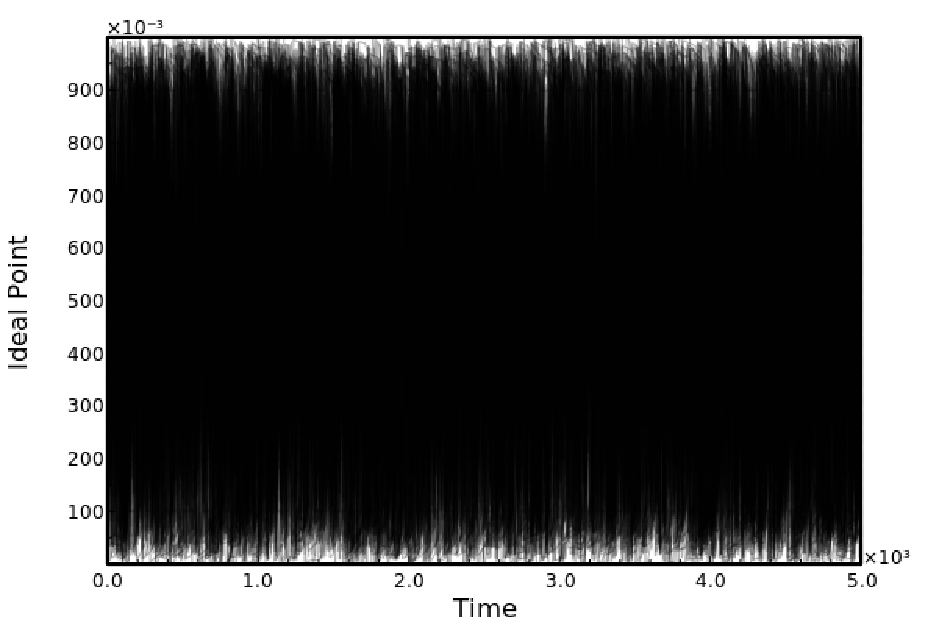
\includegraphics[scale = 0.5]{ims/rho001.pdf}
    \caption{\(\rho = 0.01\)}
  \end{figure}
\end{frame}



\begin{frame}{Resultados Parciais - Sobre \(\rho\)}
Quando \(n = 5 \text{ ou } 10\) ainda domina, mas num espaço menor.
Quanto maior  \(\sigma\) e \(p\) menor o espaço.  

\end{frame}


\begin{frame}{Resultados Parciais - Sobre \(\rho\), com \(n = 10 \)}
  
  \begin{figure}[H]
    \centering
    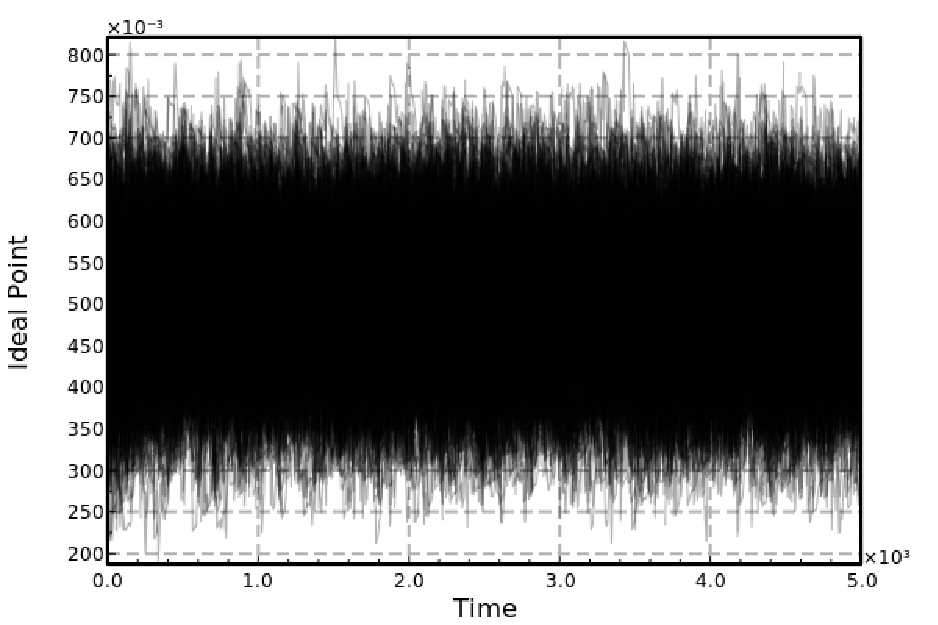
\includegraphics[scale = 0.5]{ims/p01sigma03rho01.pdf}
    \caption{\(\rho = 0.1\)  ; \(p = 0.1\); \(\sigma = 0.3\) }
  \end{figure}
\end{frame}


\begin{frame}{Resultados Parciais - Sobre \(\rho\), com \(n = 10 \)}
  
  \begin{figure}[H]
    \centering
    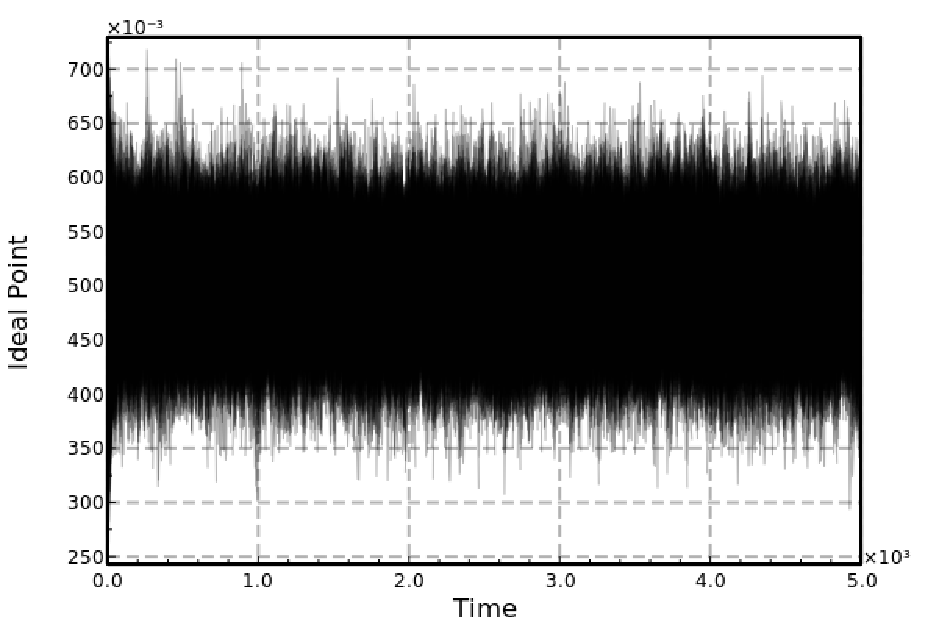
\includegraphics[scale = 0.5]{ims/p09sigma03rho01.pdf}
    \caption{\(\rho = 0.1\)  ; \(p = 0.9\); \(\sigma = 0.3\) }
  \end{figure}
\end{frame}

\begin{frame}{Resultados Parciais - Sobre \(\rho\), com \(n = 10 \)}
  
  \begin{figure}[H]
    \centering
    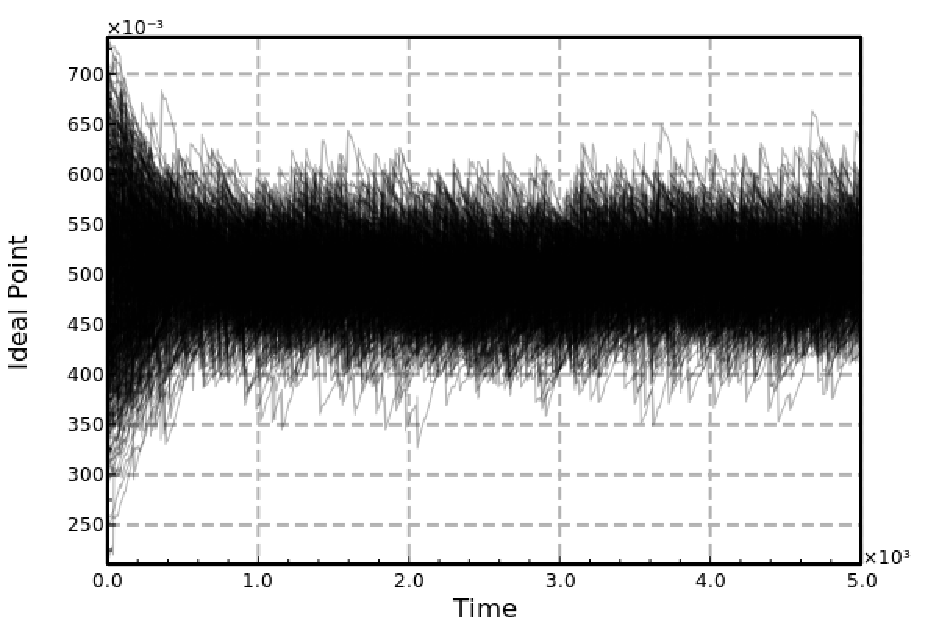
\includegraphics[scale = 0.5]{ims/p01sigma03rho001.pdf}
    \caption{\(\rho = 0.01\)  ; \(p = 0.1\); \(\sigma = 0.3\) }
  \end{figure}
\end{frame}


\begin{frame}{Resultados Parciais - Sobre \(\rho\), com \(n = 10 \)}
  \begin{figure}[H]
    \centering
    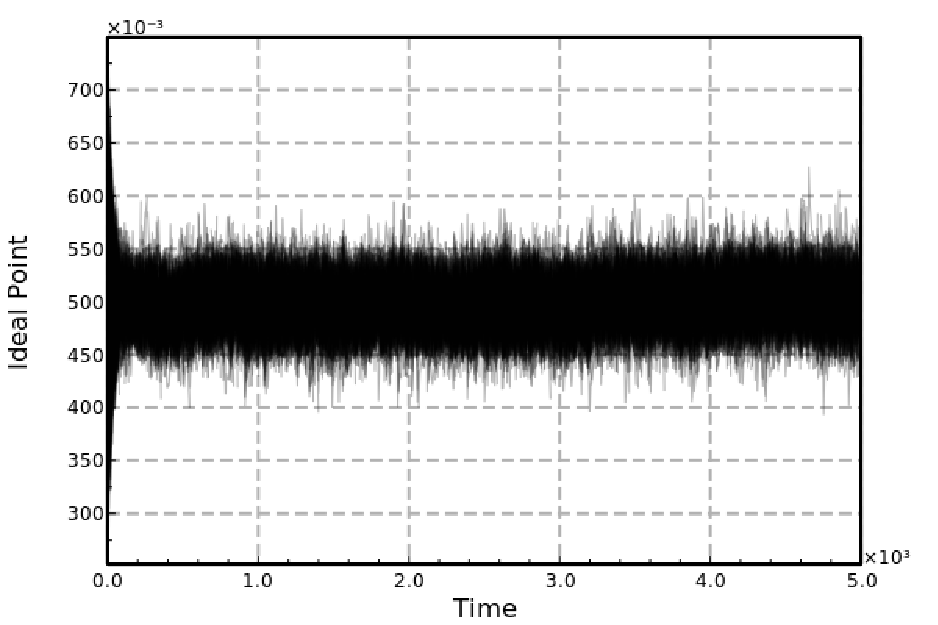
\includegraphics[scale = 0.5]{ims/p09sigma03rho001.pdf}
    \caption{\(\rho = 0.01\)  ; \(p = 0.9\); \(\sigma = 0.3\) }
  \end{figure}
\end{frame}


\begin{frame}{Resultados Parciais - Sobre \(n\), com \(\rho = 0 \) ou 0.0001}
  Aumentar o \(n\) faz aumentar o número de clusters, e os torna mais robustos
  ao ruído.
\end{frame}

\begin{frame}{Resultados Parciais - Sobre \(n\), com \(\rho = 0 \) ou 0.0001}
  \begin{figure}[H]
    \centering
    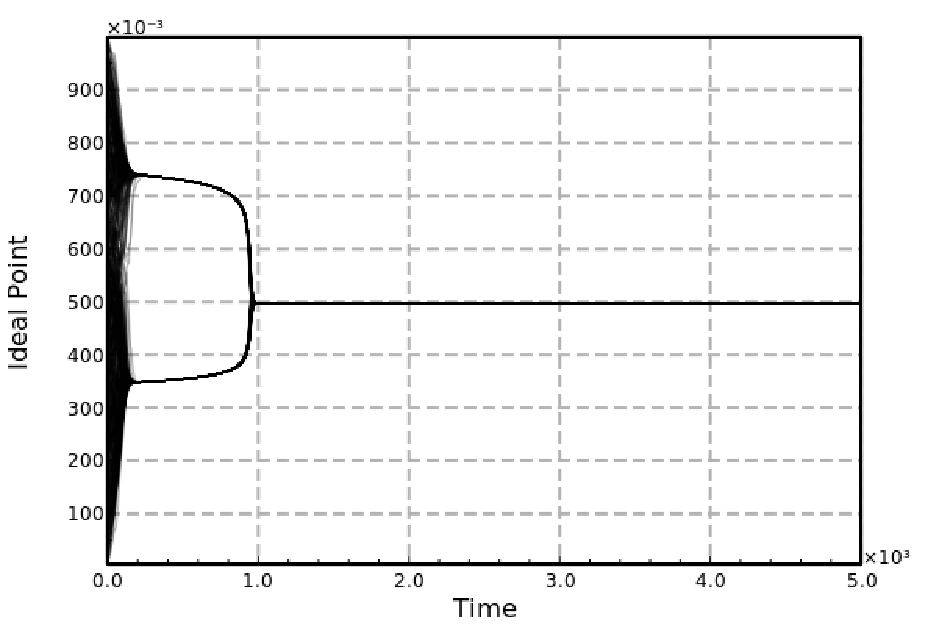
\includegraphics[scale = 0.5]{ims/p(01)sigma(01)rho(00).pdf}
    \caption{\(n = 1\) ; \(\rho = 0.0\)  ; \(p = 0.1\); \(\sigma = 0.1\) }
  \end{figure}
\end{frame}





\begin{frame}{Resultados Parciais - Sobre \(n\), com \(\rho = 0 \) ou 0.0001}
  \begin{figure}[H]
    \centering
    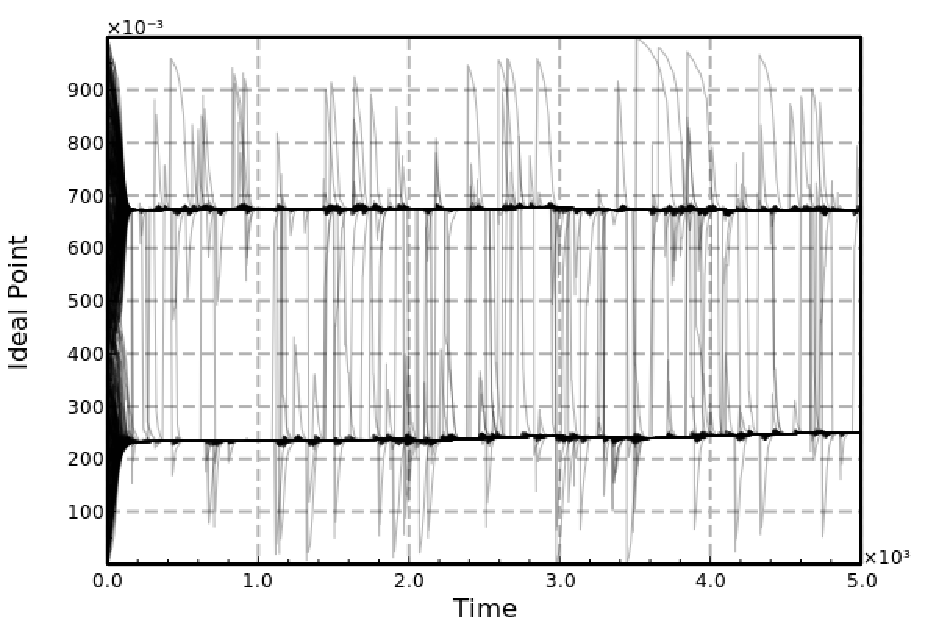
\includegraphics[scale = 0.5]{ims/p(01)sigma(01)rho(00001).pdf}
    \caption{ \(n = 1 \); \(\rho = 0.0001\)  ; \(p = 0.1\); \(\sigma = 0.1\) }
  \end{figure}
\end{frame}

\begin{frame}{Resultados Parciais - Sobre \(n\), com \(\rho = 0 \) ou 0.0001}
  \begin{figure}[H]
    \centering
    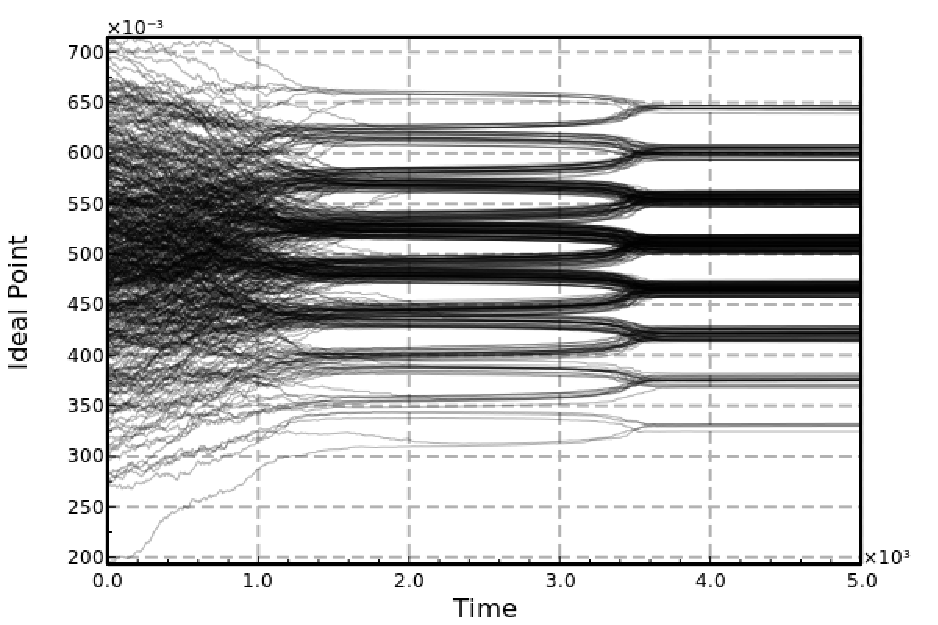
\includegraphics[scale = 0.5]{ims/n10p(01)sigma(01)rho(00).pdf}
    \caption{\(n = 10\) ; \(\rho = 0.0\)  ; \(p = 0.1\); \(\sigma = 0.1\) }
  \end{figure}
\end{frame}

\begin{frame}{Resultados Parciais - Sobre \(n\), com \(\rho = 0 \) ou 0.0001}
  \begin{figure}[H]
    \centering
    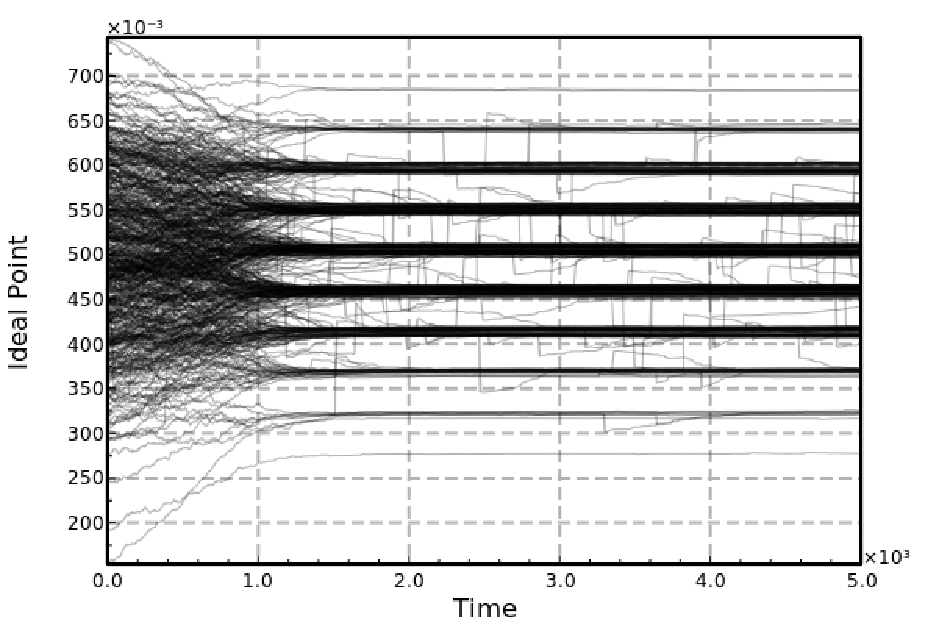
\includegraphics[scale = 0.5]{ims/n10p(01)sigma(01)rho(00001).pdf}
    \caption{ \(n = 10 \); \(\rho = 0.0001\)  ; \(p = 0.1\); \(\sigma = 0.1\) }
  \end{figure}
\end{frame}




\section*{Referências}
\begin{frame}[allowframebreaks]{Referências}
\printbibliography[heading=none]
\end{frame}

\end{document} 
%%% Local Variables:
%%% mode: latex
%%% TeX-master: ""
%%% End:
